\section{Physik}
\subsection{College Physics II}
\subsection{College Physics Experiment I}

\subsubsection{Wheatstone bridge}

\begin{figure}
  \centering
  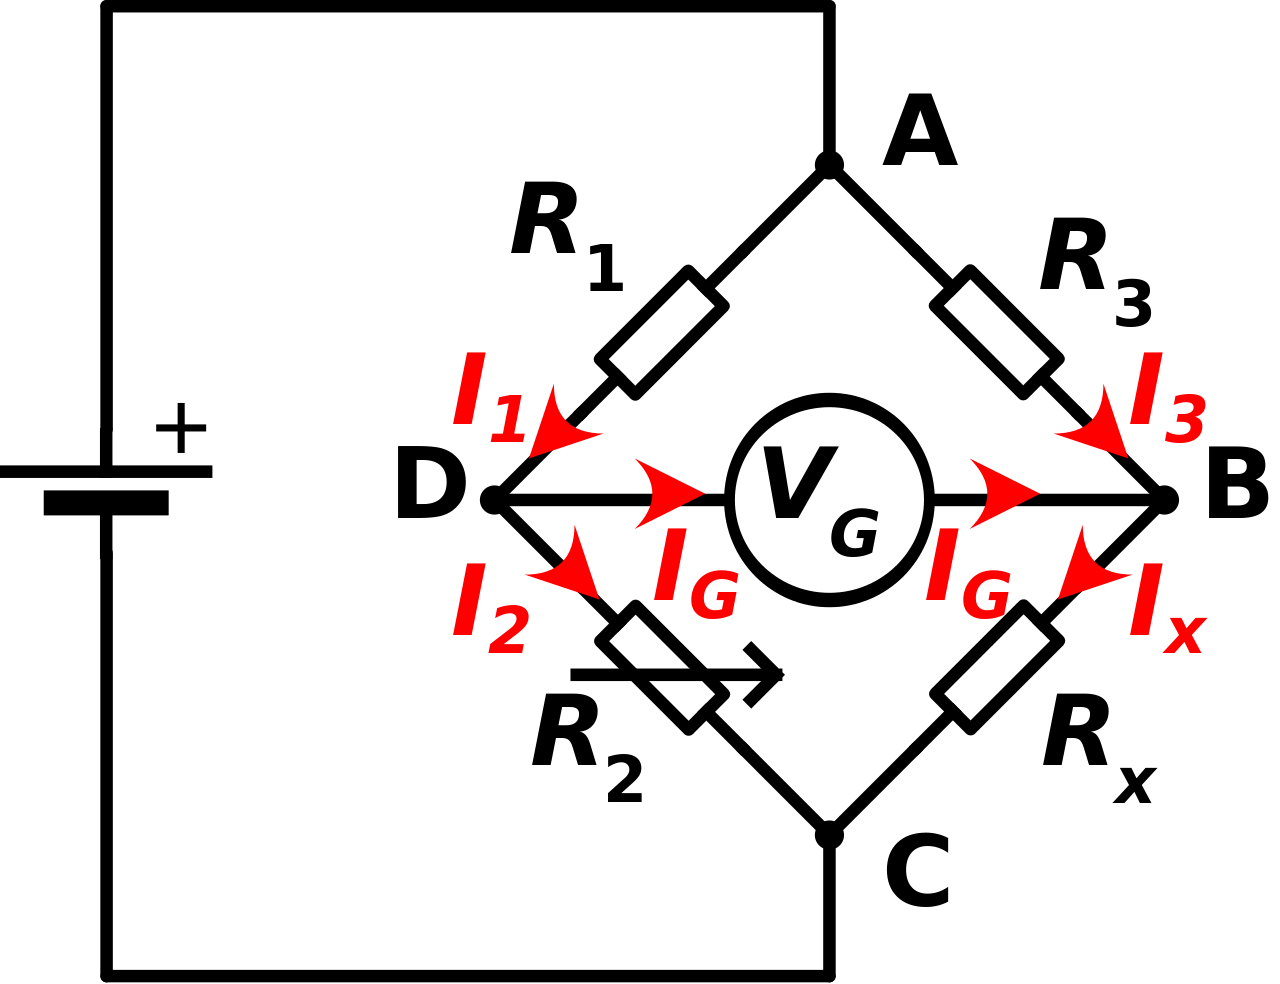
\includegraphics[width=2.5in]{fig/1280px-Wheatstonebridge_current.svg.png}
  \caption{Wheatstone bridge}\label{fig_wheatstonebridge}
\end{figure}

A Wheatstone bridge is an electrical circuit used to measure an unknown electrical resistance by balancing two legs of a bridge circuit, one leg of which includes the unknown component. The primary benefit of a wheatstone bridge is its ability to provide extremely accurate measurements.

From Kirchhoff's Current Law:

\begin{multline*}
  I_3-I_x+I_G=0 \\
  I_1-I_2-I_G=0
\end{multline*}

And from Kirchhoff's Voltage Law:

\begin{multline*}
  (I_3\dot R_3)-(I_G\dot R_G)-(I_1\dot R_1)=0 \\
  (I_x\dot R_x)-(I_2\dot R_2)+(I_G\dot R_G)=0
\end{multline*}

when the bridge is balanced, then $I_G=0$, then

$$
R_x=\frac{R_2\dot I_2\dot I_3\dot R_3}{R_1\dot I_1\dot I_x}
$$

and thus:

$$R_x=\frac{R_3 \dot R_2}{R_1}$$

\subsubsection{Thermocouple}

\paragraph{Seebeck effect} When two dissimilar metals are joined at one end, an electrical potential
called the ``Seebeck voltage'' is generated, which changes proportionally to changes in the temperature at the joint.

\subsection{Basis of Microwave Technique}
The first part of the course reviews the fundamental of electromagnetic, the Maxwell's Equation. Then focus on the basis of microwave technique, which is about Transmission Line, Waveguide, and lastly S-parameters.
\subsubsection{Maxwell's Equation}

All electromagnetic behaviors can ultimately be explained by Maxwell’s four basic equations:
\begin{align*}
  \mbox{Gauss's law   } \nabla \cdot \mathbf{E} &= \frac{\rho}{\varepsilon_0} \\
  \mbox{Gauss's law for magnetism   } \nabla \cdot \mathbf{B} &= 0 \\
  \mbox{Faraday's law of inducton   } \nabla \times \mathbf{E} &= - \frac{\partial \mathbf{B}}{\partial t} \\
  \mbox{Apm\`ere's cicuital law   } \nabla \times \mathbf{B} &= \mu(\mathbf{J}+\varepsilon\frac{\partial \mathbf{E}}{\partial t})
\end{align*}
\subsubsection{Transmission Line}
A transmission line is a specialized cable designed to carry alternating current of radio frequency.
Types of transmission line include parallel line (ladder line, twisted pair), coaxial cable, stripline, and microstrip. Transmission lines become necessary when the length of the cable is longer than a significant fraction of the transmitted frequency's wavelength.

\paragraph{Telegrapher's equations} The telegrapher's equations are a pair of linear differential equations which describe the voltage and current on an electrical transmission line with distance and time
\begin{align*}
  \frac{\partial V(x)}{\partial x} &= -(R+j\omega L)I(x) \\
  \frac{\partial I(x)}{\partial x} &= -(G+j\omega C)V(x)
\end{align*}

Steady-state Telegrapher's equations are:

\begin{align*}
  \frac{\partial ^2 V(x)}{\partial x^2} &= \gamma ^2 LC \cdot V(x) \\
  \frac{\partial ^2 I(x)}{\partial x^2} &= \gamma ^2 LC \cdot I(x)
\end{align*}

where propagation constant $\gamma = \sqrt{(R+j\omega L)(G+j\omega C)} = \alpha + j \beta$.

The real part of the propagation constant is the \emph{attenuation constant}. It causes a signal amplitude to decrease along a transmission line. The \emph{phase constant} is denoted by $\beta = 2\pi / \lambda$. It determines the sinusoidal amplitude/phase of the signal along a transmission line, at a constant time.

\subparagraph{Phase constant versus wavenumber} Phase constant and wavenumber are often treated as the same thing. Indeed, for TEM transmission lines (coax and stripline), the phase constant and wavenumber are equal. Wavequide is one case where you need to understand the difference between the two.

\emph{Wavenumber} is denoted by lower case ``k'', and is a measure of how many cycles a wave has in a given length, for a traveling wave that is frozen in time.

\paragraph{Characteristic impedance}
$$Z_0=\frac{U^+(z)}{I^+(z)}=\sqrt{\frac{R+j\omega L}{G+j\omega C}}$$
The characteristic impedance of a transmission line is the \emph{ratio} of the voltage and current of a wave travelling along the line. When the wave reaches the end of the line, in general, there will be a \textbf{reflected wave} which travels back along the line in the opposite direction.

When this wave reaches the source, it adds to the transmitted wave and the ratio of the voltage and current at the input to the line will no longer be the characteristic impedance. This new ratio is called the \textbf{input impedance}.

$$Z_{in}(z')=\frac{U(z')}{I(z')}=Z_0\frac{Z_l+jZ_0\tan\beta z'}{Z_0+jZ_l\tan\beta z'}$$

\paragraph{Impedance Matching}

If impedance matches, no reflection will be produced along the line, and thus input impedance equals to characteristic impedance.

Impedance matching has the following advantages:
\begin{itemize}
  \item load accepts maximum power output from matched source
  \item power losses is minimum in the matched transmission line
  \item the matched transmission line has the largest power capacity
  \item signal source operates in stable condition
\end{itemize}

\subparagraph{VSWR(Voltage Standing Wave Ratio)}
$$\textrm{reflection coefficient }\Gamma = \frac{V_r}{V_f}=\frac{Z_{in}(z')-Z_0}{Z_{in}(z')+Z_0}$$
Standing Wave Ratio (SWR) is a measure of impedance matching of loads to the characteristic impedance of a transmission line or waveguide.

$$VSWR=\frac{|V_{max}|}{|V_{min}|}=\frac{1+|\Gamma|}{1-|\Gamma|}$$

\begin{figure}
  \centering
  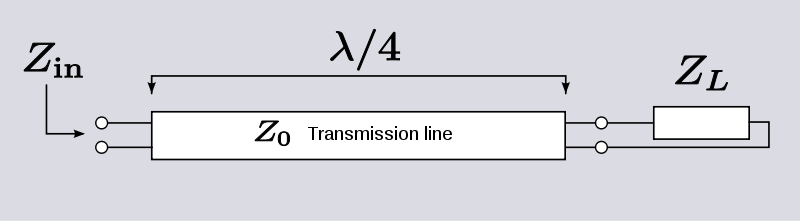
\includegraphics[width=4.2in]{fig/800px-Quarter_wave_impedance_transformer.svg.png}
  \caption{Diagram illustrating how a quarter wavelength transmission line can be used to transform an impedance into its dual.}\label{fig_quarter_wave}
\end{figure}

\subparagraph{QWT (Quarter-wave impedance transformer)} For a $\lambda /4$-length TL, the input impedance is $Z_{in}=Z_1^2 / Z_L$. Adjust $Z_1$ so that $Z_{in}=Z_0$, and find $Z_1=\sqrt{Z_0Z_L}$. By using a quarter-wavelength of transmission line, the impedance of the load ($Z_L$) can be transformed via the above equation.

In general, impedance matching is very important in RF/microwave circuit design. It is relatively simple at a single frequency, but becomes very difficult if wideband impedance matching is desired.

\subparagraph{Smith Chart} Smith chart is a graphical aid or nomogram designed for electrical and electronics engineers specializing in radio frequency (RF) engineering to assist in solving problems with transmission lines and matching circuits.

\begin{figure}
  \centering
  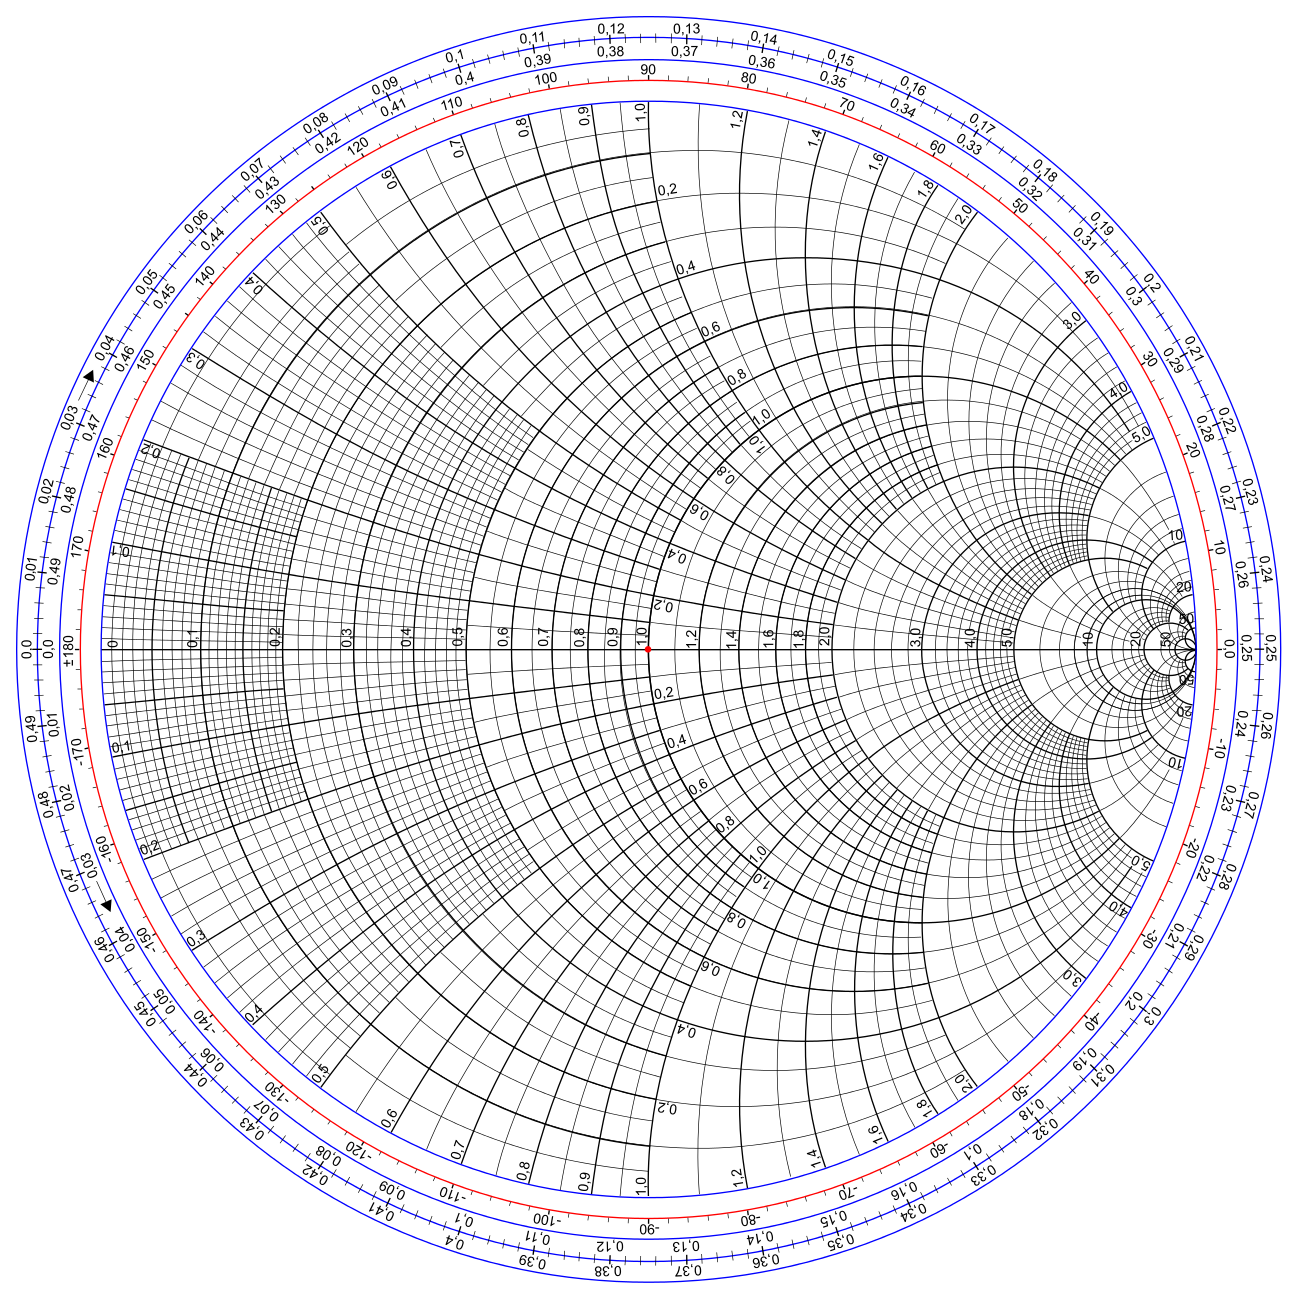
\includegraphics[width=4.5in]{fig/1300px-Smith_chart_gen.svg.png}
  \caption{Impedance Smith Chart}\label{fig_smith_chart}
\end{figure}

\subsubsection{Waveguide}
Waves propagate in all directions in open space. A waveguide confines the wave to propagate in one dimension, so that, under ideal conditions, the wave loses no power while propagating.

\paragraph{Transverse Mode}

\begin{itemize}
  \item Transverse Electric and Magnetic (TEM),
  \item Transverse Electric (TE) $E_z = 0$ and $H_z \neq 0$
  \item Transverse Magnetic (TM) $E_z \neq 0$ and $H_z = 0$
\end{itemize}

Assume that the waveguide is invariant in the z-direction, and that the wave is propagating in z as $e^{-j\beta z}$. From $\nabla \times \bar{E}=-j\omega \mu \bar{H}$, we find
$$H_x=\frac{j}{k_c^2}(\omega \varepsilon \frac{\partial E_z}{\partial y}-\beta \frac{\partial H_z}{\partial x})$$
where $k_c^2\equiv k^2-\beta ^2$ and $k^2=\omega ^2 \mu \varepsilon$.

Most important point: all transverse components of $\bar{E}$ and $\bar{H}$ can be determined from only the axial components $E_z$ and $H_z$.

\paragraph{Dominant Mode} The mode with the lowest cutoff frequency is termed the dominant mode of the guide. In rectangular and circular (hollow pipe) waveguides, the dominant modes are designated the $TE_{1,0}$ mode. Single mode operation is most often the preferred application for hollow waveguides.

$$\lambda_c=\frac{2}{\sqrt{(\frac{m}{a})^2+(\frac{n}{b})^2}}$$

\subsubsection{S-parameters}

%The scattering matrix is a mathematical construct that quantifies how RF energy propagates through a multi-port network. The S-matrix is what allows us to accurately describe the properties of incredibly complicated networks as simple ``black boxes''. For an RF signal incident on one port, some fraction of the signal bounces back out of that port, some of it scatters and exits other ports (and is perhaps even amplified), and some of it disappears as heat or even electromagnetic radiation.

\begin{figure}
  \centering
  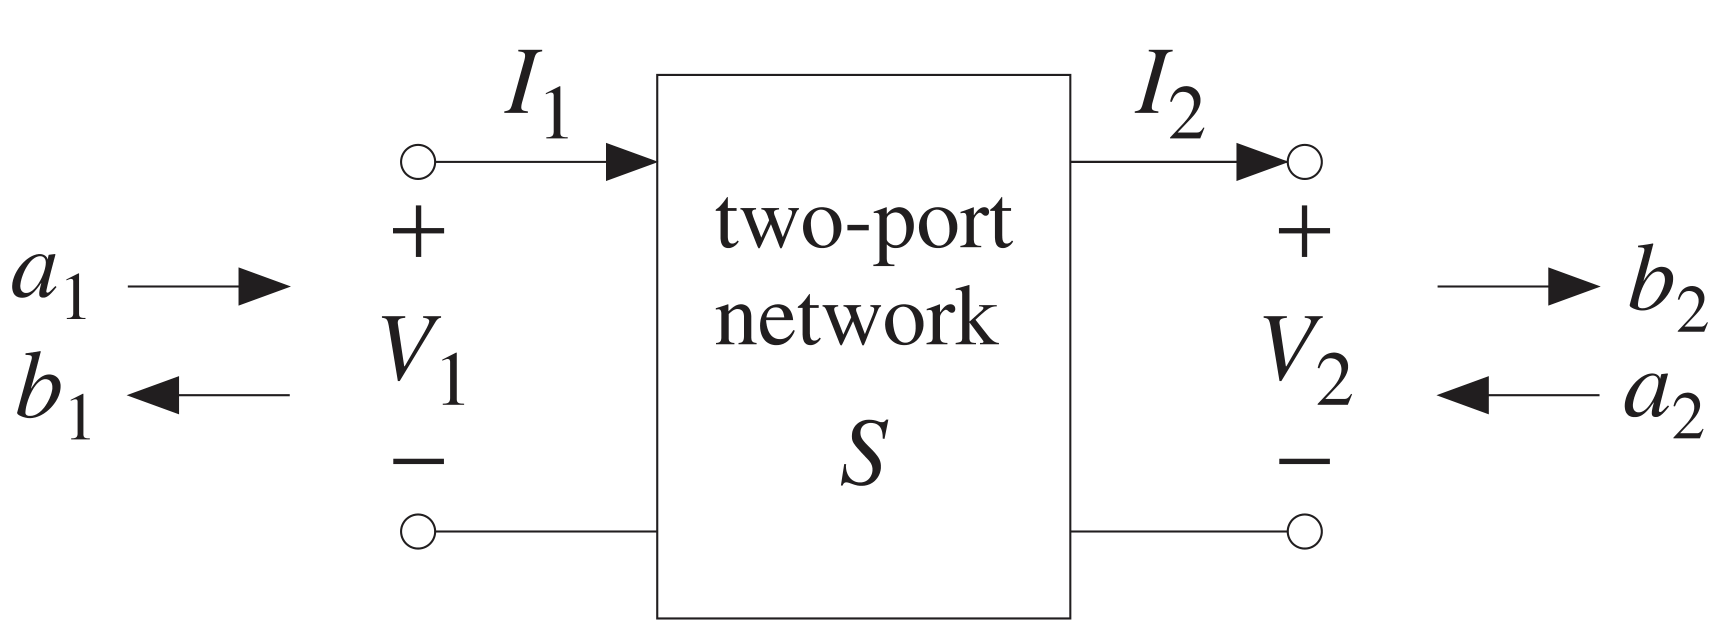
\includegraphics[width=3.2in]{fig/S_parameter.png}
  \caption{Two-port network}\label{fig_s_parameter}
\end{figure}

%\begin{align*}
%  S_{11} &= \frac{b1}{a1} \\
%  S_{12} &= \frac{b1}{a2} \\
%  S_{21} &= \frac{b2}{a1} \\
%  S_{22} &= \frac{b2}{a2}
%\end{align*}

Linear networks, or nonlinear networks operating with signals sufficiently small to cause the networks to respond in a linear manner, can be completely characterized by parameters measured at the network terminals (ports) without regard to the contents of the networks.

S-parameters are important in microwave design because they are easier to measure and work with at high frequencies than other kinds of parameters.

\[
\begin{bmatrix}
   b_1 \\
   b_2
\end{bmatrix}
=
\begin{bmatrix}
   S_{11} & S_{12} \\
   S_{21} & S_{22}
\end{bmatrix}
\begin{bmatrix}
   a_1 \\
   a_2
\end{bmatrix}
\]

The parameters $S_{11}$, $S_{22}$ have the meaning of reflection coefficients, and $S_{12}$, $S_{21}$, have the meaning of transmission coefficients.

S-parameters change with the measurement frequency, so frequency must be specified for any S-parameter measurements stated, in addition to the characteristic impedance or system impedance.

\subsection{Engineering Optics}
In this course, I've learnt the general principles of Geometric Optics, Apertures and Stops, Aberrations, and the structure of Optical Instruments.

\subsubsection{General Principles}

\paragraph{Rectilinear Propagation}
\begin{itemize}
  \item left alone, rays don't change direction
  \item rays change direction when they encounter a new medium according to Snell's Law
\end{itemize}

\paragraph{Snell's Law} When a ray of light strikes a new medium, it may be reflected or it may traverse the boundary with a change of direction(refraction).

\subparagraph{Refractive Index} The \emph{refractive index} describes how light propagates through a medium. It is defined as:

$$n=\frac{c}{v}$$

where $c$ is the speed of light, and $v$ is the phase velocity of light in the medium.

\begin{figure}
  \centering
  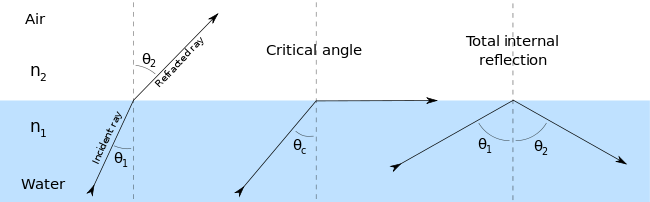
\includegraphics[width=4.5in]{fig/650px-RefractionReflextion.svg.png}
  \caption{Refraction of light at the interface between two media.}\label{fig_snell}
\end{figure}

$$n_1\textrm{sin}\theta _1 = n_2 \textrm{sin}\theta _2$$

\subparagraph{Total internal reflection} When a ray strikes a medium boundary at a larger angle than critical angle, then the ray cannot pass through and is entirely reflected.

%\paragraph{Stigmatic Condition (perfect imaging)} If a system is perfectly stigmatic for A and A', then $L(AA')=constant$.
%
%\paragraph{Refraction of a Light Ray at a Single Surface}
%
%\begin{equation*}
%\left\{
%  \begin{aligned}
%    \textrm{sin}I =& (L-r)\frac{\textrm{sin}U}{r} \\
%    \textrm{sin}I' =& \frac{n}{n'}\textrm{sin}I \\
%    U' =& U+I-I'\\
%    \frac{\textrm{sin}I'}{L'-r}=& \frac{\textrm{sin}U'}{r}
%  \end{aligned}
%\right.
%\end{equation*}
%$$\Rightarrow L'= r(1+\frac{\textrm{sin}I'}{\textrm{sin}U'})$$
%\begin{align*}
%  \mbox{laberal magnification:   } \beta &= m = \frac{y'}{y} \\
%  \mbox{longitudinal magnification:   } \alpha &=m_L= \frac{dz'}{dz} \\
%  \mbox{Helmholz invariant:   } L &=nyu=n'y'u'(paraxial marginal)
%\end{align*}
%
%\paragraph{Rays close to the optic axis:}
%$$\frac{1}{s}+\frac{1}{s'}= \frac{2}{R}$$
%
%where s is the object distance to the Kugel on the axis.

\begin{figure}
  \centering
  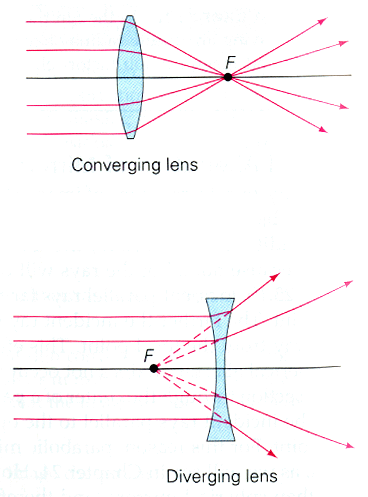
\includegraphics[width=2.7in]{fig/lenses.png}
  \caption{lens imaging}\label{fig_lens_imaging}
\end{figure}

\subsubsection{Graphical Method - Principal Ray Tracing}
\begin{itemize}
  \item an incident ray pass the 2nd focus point parallel to the optic axis.
  \item a ray through centre of lens doesn't deviate.
  \item a ray through 1st focus point refract parallel to the optical axis.
\end{itemize}

\paragraph{Principal Planes} Conjugate planes for which transverse magnification is unity ($\beta=1
$) , its intersection with axis are named \emph{principal points}.

\begin{figure}
  \centering
  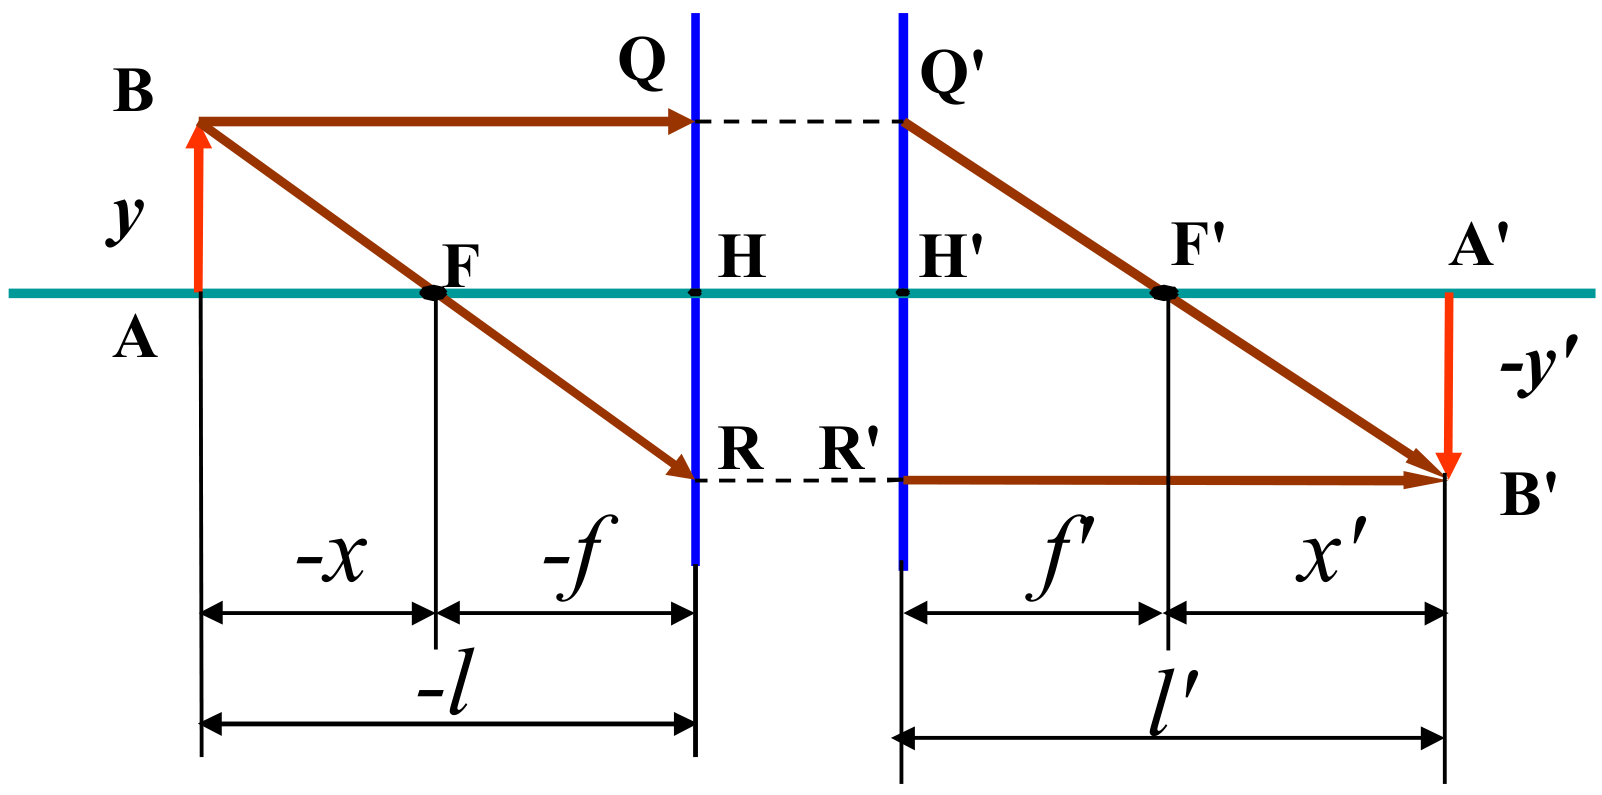
\includegraphics[width=3.2in]{fig/newtons_equation.png}
  \caption{Optical System}\label{fig_newtons_equation}
\end{figure}

\paragraph{Newton's Equation}

$$xx' =ff'$$ or $$\frac{x'}{l'}+\frac{x}{l} = 1$$

\paragraph{Gauss's Equation}

$$\frac{f'}{l'}+\frac{f}{l}=1$$

\subsubsection{Apertures and stops}

\paragraph{Chief Ray} Starts from off-axis object, goes through the cnetre of the Aperture, and marginal ray goes through the edge of the aperture.

\paragraph{Aperture}

The aperture and focal length of an optical system determine the cone angle of a bundle of rays that come to a focus in the image plane.

\begin{itemize}
  \item largest possible \emph{angle} for object of zero height
  \item depends on where the object is located
  \item determines the system resolution, light transmission efficiency, and the depth of field
\end{itemize}

NA: numerical aperture

$$NA=n\textrm{sin}\alpha $$

which is a property of cones of light.

\subparagraph{Aperture Stop} The physical element which limits the nagle of acceptance of the imaging system. The image of the \emph{aperture stop} in \emph{object} (image) space

\begin{figure}
  \centering
  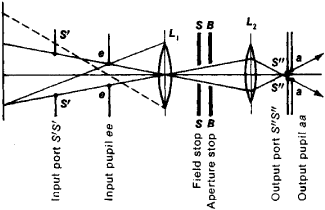
\includegraphics[width=3.0in]{fig/gsed_0001_0015_0_img3897.png}
  \caption{Aperture and stops}\label{fig_Aperture_and_stops}
\end{figure}

\subparagraph{Field Stop} The element that limits the size or angular breadth of an object that can be imaged by the system is called the field stop. For cameras, the size of the film or CCD detector determines the maximum image size and serves as the field stop. The images of the field stop is called \emph{window}. Filed stop alse defines the Field of View(FoV).

\paragraph{Depth of Field} Depth of Field is the distance between the nearest and farthest objects in a scene that appear acceptably sharp in an image.

%\begin{equation*}
%\left\{
%  \begin{aligned}
%    \delta z &=\frac{p}{NA}\\
%    \Delta &=\frac{\delta z}{\alpha}
%  \end{aligned}
%\right.
%\end{equation*}

\subsubsection{Aberrations}
\paragraph{Geometrical Aberrations}
\begin{itemize}
\item spherical aberration
\item astigmatism
\item coma
\item curvature of field
\item distortion
\end{itemize}

\begin{figure}
  \centering
  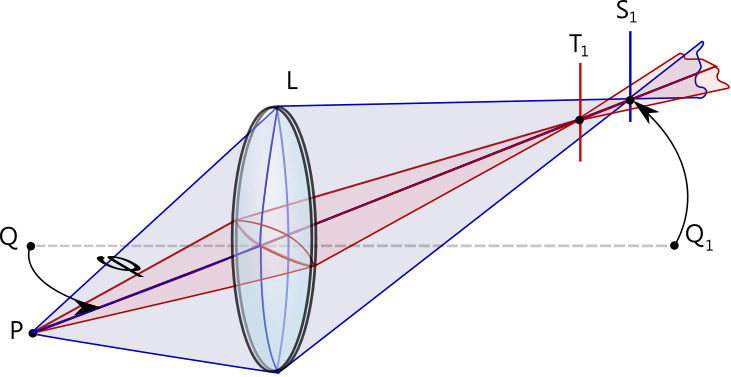
\includegraphics[width=3.0in]{fig/731px-Astigmatism.svg.png}
  \caption{astigmatism}\label{fig_astigmatism}
\end{figure}

\begin{figure}
  \centering
  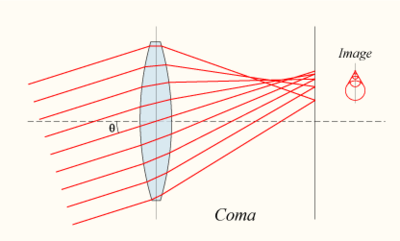
\includegraphics[width=3.0in]{fig/400px-Lens-coma.png}
  \caption{coma}\label{fig_coma}
\end{figure}

\begin{figure}
  \centering
  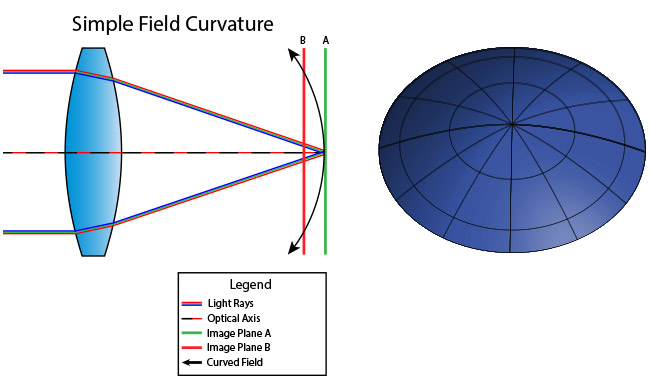
\includegraphics[width=3.0in]{fig/curvature_of_field.png}
  \caption{curvature of field}\label{fig_curvature_of_field}
\end{figure}

\begin{figure}
  \centering
  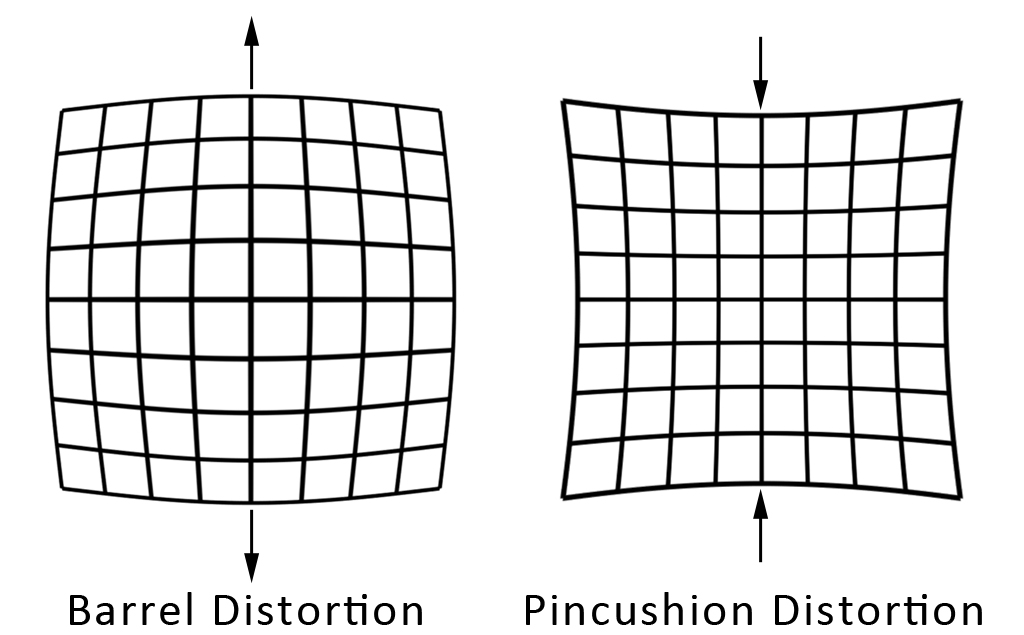
\includegraphics[width=3.0in]{fig/distortion.png}
  \caption{distortion}\label{fig_distortion}
\end{figure}

\subsubsection{Optical Instruments}

\begin{figure}
  \centering
  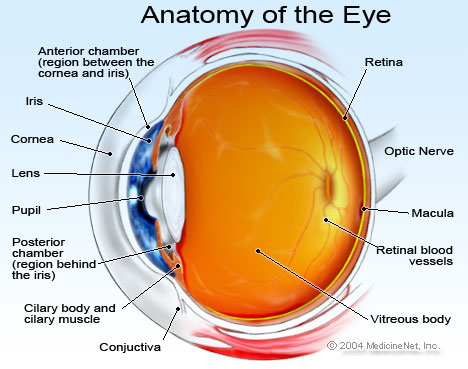
\includegraphics[width=3.0in]{fig/eye.png}
  \caption{eye}\label{fig_eye}
\end{figure}

\paragraph{Near Point} Most people cannot focus on an object that is closer than a certain distance known as the \emph{near point} ($D = 25cm$).

\begin{figure}
  \centering
  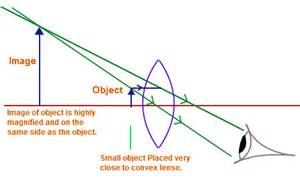
\includegraphics[width=3.0in]{fig/magnifying_glass.png}
  \caption{Magnifying Glass}\label{fig_magnifying_glass}
\end{figure}

\begin{figure}
  \centering
  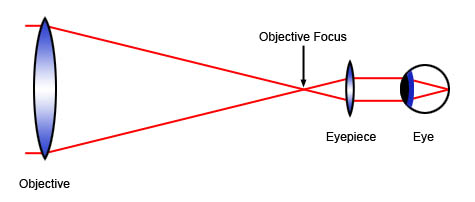
\includegraphics[width=3.0in]{fig/telescope.png}
  \caption{Telescope}\label{fig_telescope}
\end{figure}

\begin{figure}
  \centering
  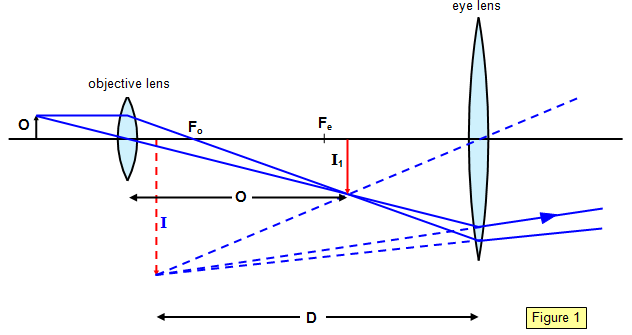
\includegraphics[width=3.0in]{fig/microscope.png}
  \caption{Microscope}\label{fig_microscope}
\end{figure}